\subsection{RC-Schaltung mit sinusförmiger Eingangsspannung}
\label{subsec:rc-schaltung-sinusfoermige-eingangsspannung}

Bisher wurde die RC-Schaltung mit einer konstanten Eingangsspannung betrachtet.
In diesem Fall lädt sich der Kondensator exponentiell auf, bis seine Spannung
den Endwert der angelegten Gleichspannung erreicht.

Nun betrachten wir den Fall, dass die Eingangsspannung nicht konstant ist,
sondern sinusförmig mit der Zeit variiert. Damit wird die Differentialgleichung
nicht mehr durch eine konstante rechte Seite angeregt, sondern durch eine
zeitabhängige Funktion.

\subsubsection{Schaltung und Eingangsspannung}
\label{subsubsec:rc-schaltung-eingangsspannung}

Wir betrachten eine RC-Reihenschaltung mit einer Eingangsspannung \(u_e(t)\).
Gesucht ist die Spannung \(u_C(t)\) am Kondensator.
\FloatBarrier
\begin{center}
	\begin{tikzpicture}[scale=1.0, european resistors]
		
		% Coordinates
		\coordinate (A) at (0,0);
		\coordinate (B) at (2,0);
		\coordinate (C) at (4,0);
		\coordinate (D) at (4,-2);
		\coordinate (E) at (0,-2);
		
		% Source
		\draw (A) to[sV, l_={$u_e(t)$}] (E);
		
		% Resistor
		\draw (A) -- (0.8,0);
		\draw (0.8,0) to[R, l={$R$}] (2.6,0);
		
		% Capacitor
		\draw (2.6,0) -- (C);
		\draw (C) to[C, l={$C$}] (D);
		
		% Ground return
		\draw (D) -- (E);
		
		% Capacitor voltage arrow
		\draw[->] (4.9,-0.2) -- (4.9,-1.8);
		\node[right] at (5.0,-1.0) {$u_C(t)$};
		
		% Current arrow
		\draw[->] (1.1,0.7) -- (2.2,0.7);
		\node[above] at (1.65,0.7) {$i(t)$};
		
	\end{tikzpicture}
\end{center}

Die Eingangsspannung sei sinusförmig:

\begin{equation}
	u_e(t) = \hat{U} \sin(\omega t).
	\label{eq:rc-eingangsspannung-sinus}
\end{equation}

Dabei ist \(\hat{U}\) der Scheitelwert der Eingangsspannung und

\begin{equation}
	\omega = 2\pi f
	\label{eq:rc-kreisfrequenz}
\end{equation}

die Kreisfrequenz.

\begin{PhysicsBox}[Physikalische Situation]
	\label{box:rc-sinus-physikalische-situation}
	Bei einer Gleichspannung nähert sich die Kondensatorspannung einem festen
	Endwert. Bei einer sinusförmigen Eingangsspannung gibt es keinen festen
	Endwert mehr. Stattdessen folgt die Kondensatorspannung der Eingangsspannung
	periodisch, jedoch mit kleinerer Amplitude und mit einer Phasenverschiebung.
\end{PhysicsBox}

\subsubsection{Aufstellung der Differentialgleichung}
\label{subsubsec:rc-sinus-differentialgleichung}

Für die Masche der Reihenschaltung gilt nach der Kirchhoffschen Maschenregel:

\begin{equation}
	u_e(t) = u_R(t) + u_C(t).
	\label{eq:rc-maschensatz}
\end{equation}

Die Spannung am Widerstand ist

\begin{equation}
	u_R(t) = R i(t).
	\label{eq:rc-widerstandsspannung}
\end{equation}

Der Strom durch den Kondensator ist

\begin{equation}
	i(t) = C \frac{du_C(t)}{dt}.
	\label{eq:rc-kondensatorstrom}
\end{equation}

Damit ergibt sich für die Spannung am Widerstand:

\begin{align}
	u_R(t)
	&= R i(t) \\[4pt]
	&= R C \frac{du_C(t)}{dt}.
	\label{eq:rc-widerstandsspannung-mit-kondensatorstrom}
\end{align}

Einsetzen in die Maschengleichung liefert:

\begin{equation}
	u_e(t)
	=
	RC \frac{du_C(t)}{dt}
	+
	u_C(t).
	\label{eq:rc-dgl-allgemein}
\end{equation}

Mit der sinusförmigen Eingangsspannung

\[
u_e(t)=\hat{U}\sin(\omega t)
\]

erhält man:

\begin{equation}
	RC \frac{du_C(t)}{dt}
	+
	u_C(t)
	=
	\hat{U}\sin(\omega t).
	\label{eq:rc-dgl-sinus}
\end{equation}

\begin{MathBox}[Differentialgleichung der RC-Schaltung bei Sinusanregung]
	\label{box:rc-dgl-sinus}
	Die Differentialgleichung der RC-Reihenschaltung mit sinusförmiger
	Eingangsspannung lautet
	
	\[
	RC \frac{du_C(t)}{dt}
	+
	u_C(t)
	=
	\hat{U}\sin(\omega t).
	\]
	
	Es handelt sich um eine lineare inhomogene Differentialgleichung erster
	Ordnung.
\end{MathBox}

\subsubsection{Normalform der Differentialgleichung}
\label{subsubsec:rc-sinus-normalform}

Teilt man Gleichung~\eqref{eq:rc-dgl-sinus} durch \(RC\), so erhält man:

\begin{equation}
	\frac{du_C(t)}{dt}
	+
	\frac{1}{RC}u_C(t)
	=
	\frac{\hat{U}}{RC}\sin(\omega t).
	\label{eq:rc-dgl-sinus-normalform}
\end{equation}

Mit der Zeitkonstante

\begin{equation}
	\tau = RC
	\label{eq:rc-zeitkonstante}
\end{equation}

wird daraus:

\begin{equation}
	\frac{du_C(t)}{dt}
	+
	\frac{1}{\tau}u_C(t)
	=
	\frac{\hat{U}}{\tau}\sin(\omega t).
	\label{eq:rc-dgl-sinus-normalform-tau}
\end{equation}

Diese Form zeigt besonders klar, dass die Zeitkonstante \(\tau\) bestimmt,
wie schnell der Kondensator auf Änderungen der Eingangsspannung reagieren kann.

\subsubsection{Vergleich mit Gleichspannungsanregung}
\label{subsubsec:rc-vergleich-gleichspannung-wechselspannung}

Bei einer konstanten Eingangsspannung \(U_0\) lautet die Differentialgleichung:

\begin{equation}
	RC \frac{du_C(t)}{dt}
	+
	u_C(t)
	=
	U_0.
	\label{eq:rc-dgl-gleichspannung}
\end{equation}

Bei sinusförmiger Eingangsspannung lautet sie dagegen:

\begin{equation}
	RC \frac{du_C(t)}{dt}
	+
	u_C(t)
	=
	\hat{U}\sin(\omega t).
	\label{eq:rc-dgl-wechselspannung-vergleich}
\end{equation}

Der Unterschied liegt nur in der rechten Seite der Differentialgleichung.
Im ersten Fall ist die Anregung konstant, im zweiten Fall zeitabhängig.

\begin{center}
	\begin{tabular}{c|c}
		Anregung & Differentialgleichung \\ \hline
		Gleichspannung & \(RC\dfrac{du_C}{dt}+u_C=U_0\) \\[8pt]
		Wechselspannung & \(RC\dfrac{du_C}{dt}+u_C=\hat{U}\sin(\omega t)\)
	\end{tabular}
\end{center}

\begin{DidacticBox}[Wichtiger Unterschied]
	\label{box:rc-gleichspannung-wechselspannung-unterschied}
	Bei Gleichspannung nähert sich die Kondensatorspannung einem konstanten
	Endwert. Bei Wechselspannung bleibt die Kondensatorspannung dauerhaft
	zeitabhängig. Nach dem Einschwingen ist sie ebenfalls sinusförmig, aber
	gegenüber der Eingangsspannung abgeschwächt und phasenverschoben.
\end{DidacticBox}

\subsubsection{Struktur der Lösung}
\label{subsubsec:rc-sinus-struktur-der-loesung}

Die Lösung der inhomogenen Differentialgleichung setzt sich aus zwei Anteilen
zusammen:

\begin{equation}
	u_C(t)
	=
	u_{C,h}(t)
	+
	u_{C,p}(t).
	\label{eq:rc-loesung-homogen-partikulaer}
\end{equation}

Dabei ist \(u_{C,h}(t)\) die Lösung der homogenen Differentialgleichung und
\(u_{C,p}(t)\) eine spezielle Lösung der inhomogenen Gleichung.

\paragraph{Homogene Lösung}

Die homogene Gleichung erhält man, indem man die rechte Seite null setzt:

\begin{equation}
	RC \frac{du_{C,h}(t)}{dt}
	+
	u_{C,h}(t)
	=
	0.
	\label{eq:rc-homogene-dgl}
\end{equation}

Ihre Lösung lautet:

\begin{equation}
	u_{C,h}(t)
	=
	K e^{-\frac{t}{RC}}.
	\label{eq:rc-homogene-loesung}
\end{equation}

Dieser Anteil beschreibt den Einschwingvorgang. Für große Zeiten verschwindet
er:

\begin{equation}
	K e^{-\frac{t}{RC}}
	\rightarrow 0
	\quad \text{für} \quad t \rightarrow \infty.
	\label{eq:rc-homogene-loesung-verschwindet}
\end{equation}

\paragraph{Partikuläre Lösung}

Die partikuläre Lösung beschreibt den dauerhaft verbleibenden sinusförmigen
Zustand. Sie besitzt dieselbe Frequenz wie die Eingangsspannung, aber eine
andere Amplitude und eine Phasenverschiebung.

Man kann sie in der Form schreiben:

\begin{equation}
	u_{C,p}(t)
	=
	\hat{U}_C \sin(\omega t - \varphi).
	\label{eq:rc-partikulaere-loesung-ansatz}
\end{equation}

Dabei ist \(\hat{U}_C\) der Scheitelwert der Kondensatorspannung und
\(\varphi\) die Phasenverschiebung gegenüber der Eingangsspannung.

\subsubsection{Stationäre Lösung}
\label{subsubsec:rc-sinus-stationaere-loesung}

Nach dem Einschwingvorgang bleibt nur die stationäre Lösung übrig. Für die
RC-Schaltung als Tiefpass ergibt sich:

\begin{equation}
	\hat{U}_C
	=
	\frac{\hat{U}}{\sqrt{1+(\omega RC)^2}}.
	\label{eq:rc-amplitude-kondensatorspannung}
\end{equation}

Die Phasenverschiebung beträgt:

\begin{equation}
	\varphi
	=
	\arctan(\omega RC).
	\label{eq:rc-phasenverschiebung}
\end{equation}

Damit lautet die stationäre Kondensatorspannung:

\begin{equation}
	u_C(t)
	=
	\frac{\hat{U}}{\sqrt{1+(\omega RC)^2}}
	\sin\left(
	\omega t
	-
	\arctan(\omega RC)
	\right).
	\label{eq:rc-stationaere-loesung}
\end{equation}

\begin{MathBox}[Stationäre Lösung des RC-Tiefpasses]
	\label{box:rc-stationaere-loesung}
	Nach dem Einschwingen lautet die Kondensatorspannung
	
	\[
	u_C(t)
	=
	\frac{\hat{U}}{\sqrt{1+(\omega RC)^2}}
	\sin\left(
	\omega t
	-
	\arctan(\omega RC)
	\right).
	\]
	
	Die Kondensatorspannung ist gegenüber der Eingangsspannung abgeschwächt und
	phasenverzögert.
\end{MathBox}

\subsubsection{Spezialfall: Frequenz von 50 Hz}
\label{subsubsec:rc-sinus-spezialfall-50hz}

Für eine Netzfrequenz von

\begin{equation}
	f = 50\,\mathrm{Hz}
	\label{eq:rc-frequenz-50hz}
\end{equation}

ergibt sich die Kreisfrequenz zu

\begin{equation}
	\omega = 2\pi f = 2\pi \cdot 50.
	\label{eq:rc-kreisfrequenz-50hz}
\end{equation}

Damit gilt näherungsweise:

\begin{equation}
	\omega \approx 314\,\mathrm{s}^{-1}.
	\label{eq:rc-kreisfrequenz-50hz-naeherung}
\end{equation}

Die Differentialgleichung lautet in diesem Fall:

\begin{equation}
	RC \frac{du_C(t)}{dt}
	+
	u_C(t)
	=
	\hat{U}\sin(314t).
	\label{eq:rc-dgl-50hz}
\end{equation}

Oder in Normalform:

\begin{equation}
	\frac{du_C(t)}{dt}
	+
	\frac{1}{RC}u_C(t)
	=
	\frac{\hat{U}}{RC}\sin(314t).
	\label{eq:rc-dgl-50hz-normalform}
\end{equation}

\begin{DidacticBox}[Einordnung]
	\label{box:rc-sinus-einordnung}
	Die RC-Schaltung bleibt auch bei sinusförmiger Eingangsspannung eine
	Differentialgleichung erster Ordnung. Der Unterschied zur Gleichspannung liegt
	nicht in der Ordnung der Gleichung, sondern in der Anregung: Die rechte Seite
	ist nun eine sinusförmige Funktion der Zeit.
\end{DidacticBox}

\subsubsection{Ergebnis}
\label{subsubsec:rc-sinus-ergebnis}

Die allgemeine Differentialgleichung der RC-Schaltung lautet:

\begin{equation}
	\boxed{
		RC \frac{du_C(t)}{dt}
		+
		u_C(t)
		=
		u_e(t)
	}
	\label{eq:rc-dgl-allgemein-ergebnis}
\end{equation}

Für eine sinusförmige Eingangsspannung

\[
u_e(t)=\hat{U}\sin(\omega t)
\]

wird daraus:

\begin{equation}
	\boxed{
		RC \frac{du_C(t)}{dt}
		+
		u_C(t)
		=
		\hat{U}\sin(\omega t)
	}
	\label{eq:rc-dgl-sinus-ergebnis}
\end{equation}

Die Lösung besteht aus einem abklingenden Einschwinganteil und einem dauerhaft
verbleibenden sinusförmigen Anteil:

\begin{equation}
	u_C(t)
	=
	K e^{-\frac{t}{RC}}
	+
	\frac{\hat{U}}{\sqrt{1+(\omega RC)^2}}
	\sin\left(
	\omega t
	-
	\arctan(\omega RC)
	\right).
	\label{eq:rc-gesamte-loesung}
\end{equation}

\begin{DidacticBox}[Merksatz]
	\label{box:rc-sinus-merksatz}
	Eine RC-Schaltung mit sinusförmiger Eingangsspannung wird durch eine
	inhomogene Differentialgleichung erster Ordnung beschrieben:
	
	\[
	RC\dot{u}_C + u_C = \hat{U}\sin(\omega t).
	\]
	
	Der exponentielle Anteil beschreibt das Einschwingen. Nach längerer Zeit
	bleibt nur die sinusförmige stationäre Lösung übrig.
\end{DidacticBox}


\subsubsection{Herleitung des dauerhaft verbleibenden sinusförmigen Anteils}
\label{subsubsec:rc-herleitung-stationaerer-sinusanteil}

Die Differentialgleichung der RC-Schaltung bei sinusförmiger Eingangsspannung
lautet

\begin{equation}
	RC \frac{du_C(t)}{dt} + u_C(t)
	=
	\hat{U}\sin(\omega t).
	\label{eq:rc-dgl-sinus-stationaer-ausgangspunkt}
\end{equation}

Mit der Zeitkonstante

\begin{equation}
	\tau = RC
	\label{eq:rc-zeitkonstante-stationaer}
\end{equation}

kann man die Gleichung kompakter schreiben als

\begin{equation}
	\tau \dot{u}_C(t) + u_C(t)
	=
	\hat{U}\sin(\omega t).
	\label{eq:rc-dgl-sinus-tau-form}
\end{equation}

Gesucht ist nun der Anteil der Lösung, der nach dem Einschwingvorgang dauerhaft
übrig bleibt. Da die Anregung sinusförmig ist und die RC-Schaltung linear ist,
erwarten wir im stationären Zustand wieder eine sinusförmige Spannung derselben
Frequenz. Allerdings können Amplitude und Phase verändert sein.

\begin{DidacticBox}[Grundidee des Ansatzes]
	\label{box:rc-grundidee-stationaerer-ansatz}
	Eine lineare RC-Schaltung erzeugt aus einer sinusförmigen Eingangsspannung
	keine neue Frequenz. Im eingeschwungenen Zustand bleibt die Frequenz gleich.
	Geändert werden nur Amplitude und Phase.
\end{DidacticBox}

Mathematisch ist es zweckmäßig, den stationären Anteil zunächst als Kombination
aus Sinus und Cosinus anzusetzen:

\begin{equation}
	u_{C,p}(t)
	=
	A\sin(\omega t) + B\cos(\omega t).
	\label{eq:rc-partikulaerer-ansatz-sinus-cosinus}
\end{equation}

Der Index \(p\) steht dabei für die partikuläre Lösung, also für eine spezielle
Lösung der inhomogenen Differentialgleichung.

Die Ableitung lautet:

\begin{align}
	\dot{u}_{C,p}(t)
	&=
	\frac{d}{dt}
	\left[
	A\sin(\omega t) + B\cos(\omega t)
	\right] \\[4pt]
	&=
	A\omega\cos(\omega t)
	-
	B\omega\sin(\omega t).
	\label{eq:rc-ableitung-partikulaerer-ansatz}
\end{align}

Nun setzen wir Ansatz und Ableitung in Gleichung~\eqref{eq:rc-dgl-sinus-tau-form}
ein:

\begin{equation}
	\tau
	\left[
	A\omega\cos(\omega t)
	-
	B\omega\sin(\omega t)
	\right]
	+
	A\sin(\omega t)
	+
	B\cos(\omega t)
	=
	\hat{U}\sin(\omega t).
	\label{eq:rc-einsetzen-partikulaerer-ansatz}
\end{equation}

Jetzt werden die Sinus- und Cosinus-Anteile gesammelt. Für die Sinus-Anteile
erhält man

\begin{equation}
	A\sin(\omega t)
	-
	\tau B\omega\sin(\omega t)
	=
	\left(A-\omega\tau B\right)\sin(\omega t).
	\label{eq:rc-sinus-anteile}
\end{equation}

Für die Cosinus-Anteile erhält man

\begin{equation}
	\tau A\omega\cos(\omega t)
	+
	B\cos(\omega t)
	=
	\left(\omega\tau A+B\right)\cos(\omega t).
	\label{eq:rc-cosinus-anteile}
\end{equation}

Damit wird Gleichung~\eqref{eq:rc-einsetzen-partikulaerer-ansatz} zu

\begin{equation}
	\left(A-\omega\tau B\right)\sin(\omega t)
	+
	\left(\omega\tau A+B\right)\cos(\omega t)
	=
	\hat{U}\sin(\omega t).
	\label{eq:rc-koeffizientenvergleich-ausgangspunkt}
\end{equation}

Auf der rechten Seite gibt es nur einen Sinus-Anteil und keinen Cosinus-Anteil.
Daher müssen die Koeffizienten vor Sinus und Cosinus einzeln übereinstimmen:

\begin{align}
	A-\omega\tau B &= \hat{U},
	\label{eq:rc-koeffizientenvergleich-sinus} \\[4pt]
	\omega\tau A+B &= 0.
	\label{eq:rc-koeffizientenvergleich-cosinus}
\end{align}

Aus Gleichung~\eqref{eq:rc-koeffizientenvergleich-cosinus} folgt

\begin{equation}
	B = -\omega\tau A.
	\label{eq:rc-b-in-abhaengigkeit-von-a}
\end{equation}

Einsetzen in Gleichung~\eqref{eq:rc-koeffizientenvergleich-sinus} ergibt

\begin{align}
	A-\omega\tau(-\omega\tau A)
	&=
	\hat{U}
	\\[4pt]
	A+(\omega\tau)^2A
	&=
	\hat{U}
	\\[4pt]
	A\left[1+(\omega\tau)^2\right]
	&=
	\hat{U}.
	\label{eq:rc-bestimmung-von-a}
\end{align}

Damit ist

\begin{equation}
	A
	=
	\frac{\hat{U}}{1+(\omega\tau)^2}.
	\label{eq:rc-koeffizient-a}
\end{equation}

Für \(B\) folgt daraus

\begin{align}
	B
	&=
	-\omega\tau A
	\\[4pt]
	&=
	-\omega\tau
	\frac{\hat{U}}{1+(\omega\tau)^2}
	\\[4pt]
	&=
	-\frac{\omega\tau\hat{U}}{1+(\omega\tau)^2}.
	\label{eq:rc-koeffizient-b}
\end{align}

Damit lautet die partikuläre Lösung zunächst

\begin{equation}
	u_{C,p}(t)
	=
	\frac{\hat{U}}{1+(\omega\tau)^2}\sin(\omega t)
	-
	\frac{\omega\tau\hat{U}}{1+(\omega\tau)^2}\cos(\omega t).
	\label{eq:rc-partikulaere-loesung-sinus-cosinus}
\end{equation}

Diese Form ist mathematisch korrekt, aber noch nicht besonders anschaulich.
Man möchte sie als einzelnen Sinus mit Amplitude und Phasenverschiebung
schreiben:

\begin{equation}
	u_{C,p}(t)
	=
	\hat{U}_C\sin(\omega t-\varphi).
	\label{eq:rc-partikulaere-loesung-amplitude-phase-ansatz}
\end{equation}

Dazu verwendet man das Additionstheorem

\begin{equation}
	\sin(\omega t-\varphi)
	=
	\sin(\omega t)\cos\varphi
	-
	\cos(\omega t)\sin\varphi.
	\label{eq:rc-additionstheorem-sinus}
\end{equation}

Damit wird

\begin{equation}
	\hat{U}_C\sin(\omega t-\varphi)
	=
	\hat{U}_C\cos\varphi \, \sin(\omega t)
	-
	\hat{U}_C\sin\varphi \, \cos(\omega t).
	\label{eq:rc-amplitude-phase-ausmultipliziert}
\end{equation}

Vergleicht man dies mit

\begin{equation}
	u_{C,p}(t)=A\sin(\omega t)+B\cos(\omega t),
	\label{eq:rc-vergleich-sinus-cosinus-form}
\end{equation}

so erhält man

\begin{align}
	A &= \hat{U}_C\cos\varphi,
	\label{eq:rc-a-amplitude-phase} \\[4pt]
	B &= -\hat{U}_C\sin\varphi.
	\label{eq:rc-b-amplitude-phase}
\end{align}

Die Amplitude ergibt sich daher aus

\begin{equation}
	\hat{U}_C
	=
	\sqrt{A^2+B^2}.
	\label{eq:rc-amplitude-aus-a-b}
\end{equation}

Einsetzen von \(A\) und \(B\) liefert

\begin{align}
	\hat{U}_C
	&=
	\sqrt{
		\left(
		\frac{\hat{U}}{1+(\omega\tau)^2}
		\right)^2
		+
		\left(
		\frac{\omega\tau\hat{U}}{1+(\omega\tau)^2}
		\right)^2
	}
	\\[6pt]
	&=
	\frac{\hat{U}}{1+(\omega\tau)^2}
	\sqrt{1+(\omega\tau)^2}
	\\[6pt]
	&=
	\frac{\hat{U}}{\sqrt{1+(\omega\tau)^2}}.
	\label{eq:rc-stationaere-amplitude-herleitung}
\end{align}

Für die Phase gilt

\begin{equation}
	\tan\varphi
	=
	\frac{\hat{U}_C\sin\varphi}{\hat{U}_C\cos\varphi}
	=
	\frac{-B}{A}.
	\label{eq:rc-tangens-phase}
\end{equation}

Mit den berechneten Werten für \(A\) und \(B\) erhält man

\begin{align}
	\tan\varphi
	&=
	\frac{
		\frac{\omega\tau\hat{U}}{1+(\omega\tau)^2}
	}{
		\frac{\hat{U}}{1+(\omega\tau)^2}
	}
	\\[6pt]
	&=
	\omega\tau.
	\label{eq:rc-tangens-phase-omega-tau}
\end{align}

Also ist

\begin{equation}
	\varphi
	=
	\arctan(\omega\tau).
	\label{eq:rc-phase-stationaer}
\end{equation}

Damit lautet der dauerhaft verbleibende sinusförmige Anteil

\begin{equation}
	u_{C,p}(t)
	=
	\frac{\hat{U}}{\sqrt{1+(\omega\tau)^2}}
	\sin\left(
	\omega t
	-
	\arctan(\omega\tau)
	\right).
	\label{eq:rc-stationaerer-anteil-tau}
\end{equation}

Da \(\tau = RC\) ist, folgt schließlich

\begin{equation}
	\boxed{
		u_{C,p}(t)
		=
		\frac{\hat{U}}{\sqrt{1+(\omega RC)^2}}
		\sin\left(
		\omega t
		-
		\arctan(\omega RC)
		\right)
	}
	\label{eq:rc-stationaerer-anteil-rc}
\end{equation}

\begin{MathBox}[Dauerhaft verbleibender Sinusanteil]
	\label{box:rc-dauerhaft-verbleibender-sinusanteil}
	Nach dem Einschwingvorgang bleibt bei sinusförmiger Eingangsspannung eine
	sinusförmige Kondensatorspannung derselben Frequenz übrig:
	
	\[
	u_{C,p}(t)
	=
	\frac{\hat{U}}{\sqrt{1+(\omega RC)^2}}
	\sin\left(
	\omega t
	-
	\arctan(\omega RC)
	\right).
	\]
	
	Die Amplitude ist kleiner als die Eingangsamplitude, und die
	Kondensatorspannung hinkt der Eingangsspannung phasenmäßig hinterher.
\end{MathBox}

Die vollständige Lösung der Differentialgleichung besteht aus dem homogenen
und dem partikulären Anteil:

\begin{equation}
	u_C(t)
	=
	u_{C,h}(t)
	+
	u_{C,p}(t).
	\label{eq:rc-vollstaendige-loesung-h-p}
\end{equation}

Der homogene Anteil lautet

\begin{equation}
	u_{C,h}(t)
	=
	K e^{-\frac{t}{RC}}.
	\label{eq:rc-homogener-anteil-erneut}
\end{equation}

Dieser Anteil beschreibt nur den Einschwingvorgang. Für große Zeiten
verschwindet er:

\begin{equation}
	K e^{-\frac{t}{RC}}
	\rightarrow 0
	\quad \text{für} \quad t \rightarrow \infty.
	\label{eq:rc-homogener-anteil-verschwindet-erneut}
\end{equation}

Deshalb bleibt im eingeschwungenen Zustand nur der partikuläre Anteil übrig:

\begin{equation}
	u_C(t)
	\approx
	u_{C,p}(t)
	\quad \text{für große Zeiten}.
	\label{eq:rc-eingeschwungener-zustand}
\end{equation}

\begin{DidacticBox}[Merksatz zur stationären Lösung]
	\label{box:rc-merksatz-stationaere-loesung}
	Bei einer linearen RC-Schaltung gilt:
	
	\[
	\text{Sinus hinein} \quad \Longrightarrow \quad \text{Sinus gleicher Frequenz heraus}.
	\]
	
	Die Frequenz bleibt gleich. Geändert werden nur Amplitude und Phase.
	Der exponentielle Anteil beschreibt lediglich das Einschwingen und verschwindet
	mit der Zeit.
\end{DidacticBox}


\subsubsection{Berechnung der Phasenverschiebung}
\label{subsubsec:rc-berechnung-phasenverschiebung}

Bei einer reinen Kapazität beträgt die Phasenverschiebung zwischen Strom und
Kondensatorspannung \(90^\circ\). In einer RC-Reihenschaltung ist die Situation
jedoch anders, weil die Eingangsspannung nicht nur am Kondensator, sondern auch
am Widerstand abfällt.

Wir betrachten erneut die RC-Reihenschaltung mit der Eingangsspannung

\begin{equation}
	u_e(t)=\hat{U}\sin(\omega t)
	\label{eq:rc-phasenverschiebung-eingangsspannung}
\end{equation}

und der Kondensatorspannung \(u_C(t)\) als Ausgangsspannung.

Die stationäre Lösung für die Kondensatorspannung lautet

\begin{equation}
	u_C(t)
	=
	\frac{\hat{U}}{\sqrt{1+(\omega RC)^2}}
	\sin\left(
	\omega t
	-
	\arctan(\omega RC)
	\right).
	\label{eq:rc-stationaere-loesung-fuer-phase}
\end{equation}

Aus dieser Darstellung liest man die Phasenverschiebung direkt ab:

\begin{equation}
	\varphi
	=
	-\arctan(\omega RC).
	\label{eq:rc-phasenverschiebung-kondensator}
\end{equation}

Das Minuszeichen bedeutet, dass die Kondensatorspannung der Eingangsspannung
hinterherläuft. Der Betrag der Phasenverschiebung ist daher

\begin{equation}
	|\varphi|
	=
	\arctan(\omega RC).
	\label{eq:rc-betrag-phasenverschiebung-kondensator}
\end{equation}

Mit

\begin{equation}
	\omega = 2\pi f
	\label{eq:rc-phase-kreisfrequenz}
\end{equation}

ergibt sich

\begin{equation}
	\boxed{
		\varphi
		=
		-\arctan(2\pi f RC)
	}
	\label{eq:rc-phasenverschiebung-frequenz}
\end{equation}

\begin{MathBox}[Phasenverschiebung des RC-Tiefpasses]
	\label{box:rc-phasenverschiebung-tiefpass}
	Für eine RC-Reihenschaltung mit Ausgangsspannung am Kondensator gilt
	
	\[
	\varphi
	=
	-\arctan(\omega RC).
	\]
	
	Die Kondensatorspannung hinkt der Eingangsspannung hinterher. Der Winkel liegt
	zwischen \(0^\circ\) und \(-90^\circ\).
\end{MathBox}

\paragraph{Herleitung über den komplexen Spannungsteiler}

Die gleiche Phasenverschiebung erhält man auch über die komplexe
Wechselstromrechnung. Die Impedanz des Kondensators lautet

\begin{equation}
	Z_C
	=
	\frac{1}{j\omega C}.
	\label{eq:rc-phase-impedanz-kondensator}
\end{equation}

Mit

\begin{equation}
	\frac{1}{j}=-j
	\label{eq:rc-phase-eins-durch-j}
\end{equation}

kann man schreiben:

\begin{equation}
	Z_C
	=
	-\frac{j}{\omega C}.
	\label{eq:rc-phase-impedanz-kondensator-minus-j}
\end{equation}

Die Gesamtimpedanz der Reihenschaltung ist

\begin{equation}
	Z_\mathrm{ges}
	=
	R+Z_C
	=
	R-\frac{j}{\omega C}.
	\label{eq:rc-phase-gesamtimpedanz}
\end{equation}

Die Kondensatorspannung ergibt sich aus dem komplexen Spannungsteiler:
Da Widerstand und Kondensator in Reihe liegen, fließt durch beide Bauteile
derselbe Strom \(I\). Die gesamte Impedanz der Reihenschaltung ist daher

\begin{equation}
	Z_\mathrm{ges}
	=
	R+Z_C.
	\label{eq:rc-gesamtimpedanz-spannungsteiler}
\end{equation}

Für die Eingangsspannung gilt damit

\begin{equation}
	U_e
	=
	I\left(R+Z_C\right).
	\label{eq:rc-eingangsspannung-komplex}
\end{equation}

Die Spannung am Kondensator ist

\begin{equation}
	U_C
	=
	I Z_C.
	\label{eq:rc-kondensatorspannung-komplex}
\end{equation}

Bildet man nun das Verhältnis beider Spannungen, so kürzt sich der gemeinsame
Strom \(I\) heraus:

\begin{equation}
	\frac{U_C}{U_e}
	=
	\frac{I Z_C}{I\left(R+Z_C\right)}
	=
	\frac{Z_C}{R+Z_C}.
	\label{eq:rc-spannungsteiler-herleitung}
\end{equation}
\begin{equation}
	\frac{U_C}{U_e}
	=
	\frac{Z_C}{R+Z_C}.
	\label{eq:rc-komplexer-spannungsteiler}
\end{equation}

Einsetzen von \(Z_C\) liefert

\begin{equation}
	\frac{U_C}{U_e}
	=
	\frac{\frac{1}{j\omega C}}
	{R+\frac{1}{j\omega C}}.
	\label{eq:rc-spannungsteiler-eingesetzt}
\end{equation}

Nun multiplizieren wir Zähler und Nenner mit \(j\omega C\):

\begin{align}
	\frac{U_C}{U_e}
	&=
	\frac{
		\frac{1}{j\omega C}\cdot j\omega C
	}{
		\left(
		R+\frac{1}{j\omega C}
		\right)
		j\omega C
	}
	\\[6pt]
	&=
	\frac{1}{j\omega RC+1}.
	\label{eq:rc-uebertragungsfunktion}
\end{align}

Damit erhält man die Übertragungsfunktion des RC-Tiefpasses:

\begin{equation}
	H(j\omega)
	=
	\frac{U_C}{U_e}
	=
	\frac{1}{1+j\omega RC}.
	\label{eq:rc-tiefpass-uebertragungsfunktion}
\end{equation}

Der Nenner

\begin{equation}
	1+j\omega RC
	\label{eq:rc-nenner-komplexe-zahl}
\end{equation}

ist eine komplexe Zahl mit Realteil \(1\) und Imaginärteil \(\omega RC\).

\begin{figure}[H]
	\centering
	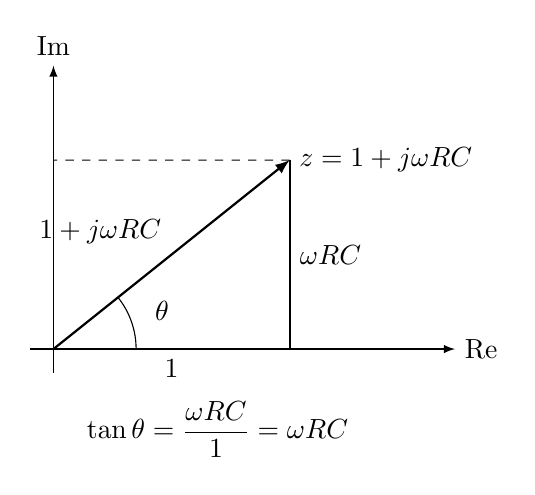
\begin{tikzpicture}[scale=3.0, >=latex]
		
		% Axes
		\draw[->] (-0.1,0) -- (1.7,0) node[right] {$\mathrm{Re}$};
		\draw[->] (0,-0.1) -- (0,1.2) node[above] {$\mathrm{Im}$};
		
		% Points and vector
		\coordinate (O) at (0,0);
		\coordinate (A) at (1,0);
		\coordinate (Z) at (1,0.8);
		
		% Dashed helper lines
		\draw[dashed] (Z) -- (A);
		\draw[dashed] (Z) -- (0,0.8);
		
		% Vector
		\draw[->, thick] (O) -- (Z) node[midway, above left] {$1+j\omega RC$};
		
		% Real and imaginary labels
		\draw[thick] (O) -- (A) node[midway, below] {$1$};
		\draw[thick] (A) -- (Z) node[midway, right] {$\omega RC$};
		
		% Angle
		\draw (0.35,0) arc[start angle=0,end angle=38.66,radius=0.35];
		\node at (0.46,0.16) {$\theta$};
		
		% Point label
		\node[right] at (Z) {$z=1+j\omega RC$};
		
		% Formula
		\node[below right] at (0.1,-0.18)
		{$\displaystyle \tan\theta=\frac{\omega RC}{1}=\omega RC$};
		
	\end{tikzpicture}
	\caption{Darstellung der komplexen Zahl \(1+j\omega RC\) in der komplexen Ebene.}
	\label{fig:komplexe-zahl-eins-plus-jomegaRC}
\end{figure}

Sein Winkel ist

\begin{equation}
	\theta
	=
	\arctan(\omega RC).
	\label{eq:rc-winkel-nenner}
\end{equation}

Da der Nenner im Ausdruck

\[
H(j\omega)=\frac{1}{1+j\omega RC}
\]

im Nenner steht, wird sein Winkel mit negativem Vorzeichen übernommen. Daher
ist die Phase der Übertragungsfunktion

\begin{equation}
	\arg H(j\omega)
	=
	-\arctan(\omega RC).
	\label{eq:rc-phase-uebertragungsfunktion}
\end{equation}

Damit folgt erneut:

\begin{equation}
	\boxed{
		\varphi
		=
		-\arctan(\omega RC)
	}
	\label{eq:rc-phasenverschiebung-endformel-komplex}
\end{equation}

\paragraph{Anschauliche Deutung}

Bei niedrigen Frequenzen ist

\begin{equation}
	\omega RC \ll 1.
	\label{eq:rc-phase-niedrige-frequenz}
\end{equation}

Dann gilt näherungsweise

\begin{equation}
	\arctan(\omega RC) \approx 0.
	\label{eq:rc-phase-niedrige-frequenz-naeherung}
\end{equation}

Die Kondensatorspannung folgt der Eingangsspannung fast ohne Verzögerung.

Bei der Grenzfrequenz gilt

\begin{equation}
	\omega RC = 1.
	\label{eq:rc-phase-grenzfrequenz-bedingung}
\end{equation}

Dann ist

\begin{equation}
	\varphi
	=
	-\arctan(1)
	=
	-45^\circ.
	\label{eq:rc-phase-grenzfrequenz}
\end{equation}

Die zugehörige Grenzfrequenz lautet

\begin{equation}
	f_g
	=
	\frac{1}{2\pi RC}.
	\label{eq:rc-grenzfrequenz-phase}
\end{equation}

Bei hohen Frequenzen ist

\begin{equation}
	\omega RC \gg 1.
	\label{eq:rc-phase-hohe-frequenz}
\end{equation}

Dann nähert sich die Phasenverschiebung dem Wert

\begin{equation}
	\varphi \rightarrow -90^\circ.
	\label{eq:rc-phase-hohe-frequenz-grenzwert}
\end{equation}

\begin{DidacticBox}[Warum nicht immer \texorpdfstring{\(90^\circ\)}{90 Grad}?]
	\label{box:rc-warum-nicht-immer-90-grad}
	Der Kondensator allein besitzt eine Phasenverschiebung von \(-90^\circ\)
	zwischen seiner Spannung und dem Strom. In der RC-Reihenschaltung wird jedoch
	die Eingangsspannung auf Widerstand und Kondensator aufgeteilt. Dadurch liegt
	die Phasenverschiebung zwischen Eingangsspannung und Kondensatorspannung nicht
	fest bei \(-90^\circ\), sondern hängt von der Frequenz ab:
	
	\[
	\varphi
	=
	-\arctan(\omega RC).
	\]
\end{DidacticBox}

\paragraph{Berechnung aus einer Oszilloskopmessung}

Die Phasenverschiebung kann auch direkt mit dem Oszilloskop bestimmt werden.
Dazu misst man die zeitliche Verschiebung \(\Delta t\) zwischen zwei
entsprechenden Punkten der beiden Sinuskurven, zum Beispiel zwischen zwei
Nulldurchgängen gleicher Richtung.

Die Periodendauer ist

\begin{equation}
	T=\frac{1}{f}.
	\label{eq:rc-periodendauer}
\end{equation}

Dann gilt für die Phasenverschiebung in Grad:

\begin{equation}
	\varphi
	=
	360^\circ \cdot \frac{\Delta t}{T}.
	\label{eq:rc-phase-oszilloskop-grad}
\end{equation}

In Radiant lautet die Formel:

\begin{equation}
	\varphi
	=
	2\pi \frac{\Delta t}{T}.
	\label{eq:rc-phase-oszilloskop-radiant}
\end{equation}

Wenn die Kondensatorspannung später erscheint als die Eingangsspannung, erhält
die Phase ein negatives Vorzeichen.

\begin{equation}
	\boxed{
		\varphi_C
		=
		-360^\circ \cdot \frac{\Delta t}{T}
	}
	\label{eq:rc-phase-oszilloskop-endformel}
\end{equation}

\begin{DidacticBox}[Praktischer Merksatz]
	\label{box:rc-phase-praktischer-merksatz}
	Für den RC-Tiefpass gilt:
	
	\[
	u_C(t) \text{ hinkt } u_e(t) \text{ hinterher.}
	\]
	
	Die Phasenverschiebung beträgt
	
	\[
	\varphi
	=
	-\arctan(2\pi f RC).
	\]
	
	Mit dem Oszilloskop kann man sie über die Zeitverschiebung messen:
	
	\[
	|\varphi|
	=
	360^\circ \frac{\Delta t}{T}.
	\]
\end{DidacticBox}